%\documentclass[a4paper,12pt,oneside,draft]{article}
\documentclass[a4paper,12pt,oneside]{article}

% In the original writelatex tamplate
\usepackage[english]{babel}
\usepackage[utf8]{inputenc}
\usepackage{amsmath}
\usepackage{graphicx}
\usepackage[colorinlistoftodos]{todonotes}

% By LoCigno
\usepackage{times}
\usepackage{graphicx}
\usepackage{subfigure}
\usepackage{csvsimple}
\usepackage{color}
\usepackage{url}
\usepackage{hyperref} 
\usepackage{cleveref}

% By Davide
\usepackage{comment}
\usepackage{booktabs}
\usepackage{color}

%Variables macros
\newcommand{\DefineVar}[2]{%
  \expandafter\newcommand\csname var-#1\endcsname{#2}%
} 
\newcommand{\var}[1]{\csname var-#1\endcsname}

\usepackage{courier}
\newcommand{\mono}[1]{\texttt{#1}}
%\newcommand{\mono}[1]{\texttt{\textbf{#1}}}

\title{Identification procedure for Lego Mindstorm motor}

\author{Diego Verona, Aliaksandr Siarohin, Mattia Digilio}

\date{\today}

\begin{document}
%\maketitle
\makeatletter  % populates \@title, \@author, \@date
\begin{titlepage}
      \centering
      ~~~~~~~~~~~~~\\[-30mm]
      
\includegraphics[keepaspectratio=true, width=7cm]{bg_eng_1r.jpg} \\[10mm]

     {
     \large \bfseries Master Degree in Computer Science\\[3mm] 
     Applied Robotics\\[3mm]
     AA 2015-2016
     }\\[10mm]

     %--------------------------------
     % Set the title, author, and date
     % 

     \vspace{0.5cm}
     {
     \Large \bfseries \textcolor{blue}{\@title} \par
     }
     \vspace{0.5cm}
%      {
%      \large {Group N. 1} \par
%      }
     \vspace{0.2cm}

     {\large {\@author}}
     \\ \vspace{.2cm}
     \@date

     \vspace{0.6cm}

    %-----------------------------------

\begin{abstract}

\textit{
  Report for the second assignment on Applied robotics: design and implement controller for the Lego NXT motor.\\In this report we show our controller, describe it properties and describe it digital implementation.
}


\end{abstract}

\end{titlepage}

\section{Design of continues time controller}
\subsection{Controller requirments}
The contoller should have zero stady state tracking error, overshot less than 20\% and settling time less than 0.4s. To show overshot requirment on root locus plot we use the folowing formula:
\begin{equation}
\frac{Re}{Im} = \frac{\xi}{\sqrt{1-\xi^{2}}} = \pm\frac{ln{0.2}}{\pi}
\end{equation}

To show settling time requirment, we use dominant pool aproximation:
\begin{equation}
Re = \frac{ln(\alpha)}{0.4}
\end{equation}

\subsection{Our design}
\begin{equation}
C(s) = \frac{(s+10)^2}{s(s+21)}
\end{equation}
\begin{equation}
K_c = 10
\end{equation}
You can see root locus in \cref{fig:root_locus}, and ideal responce to 1(t) \cref{fig:responce}. You can also see result of our scicoslab simulation  in \cref{fig:simulation}.

\begin{figure}[t]
	\centering
	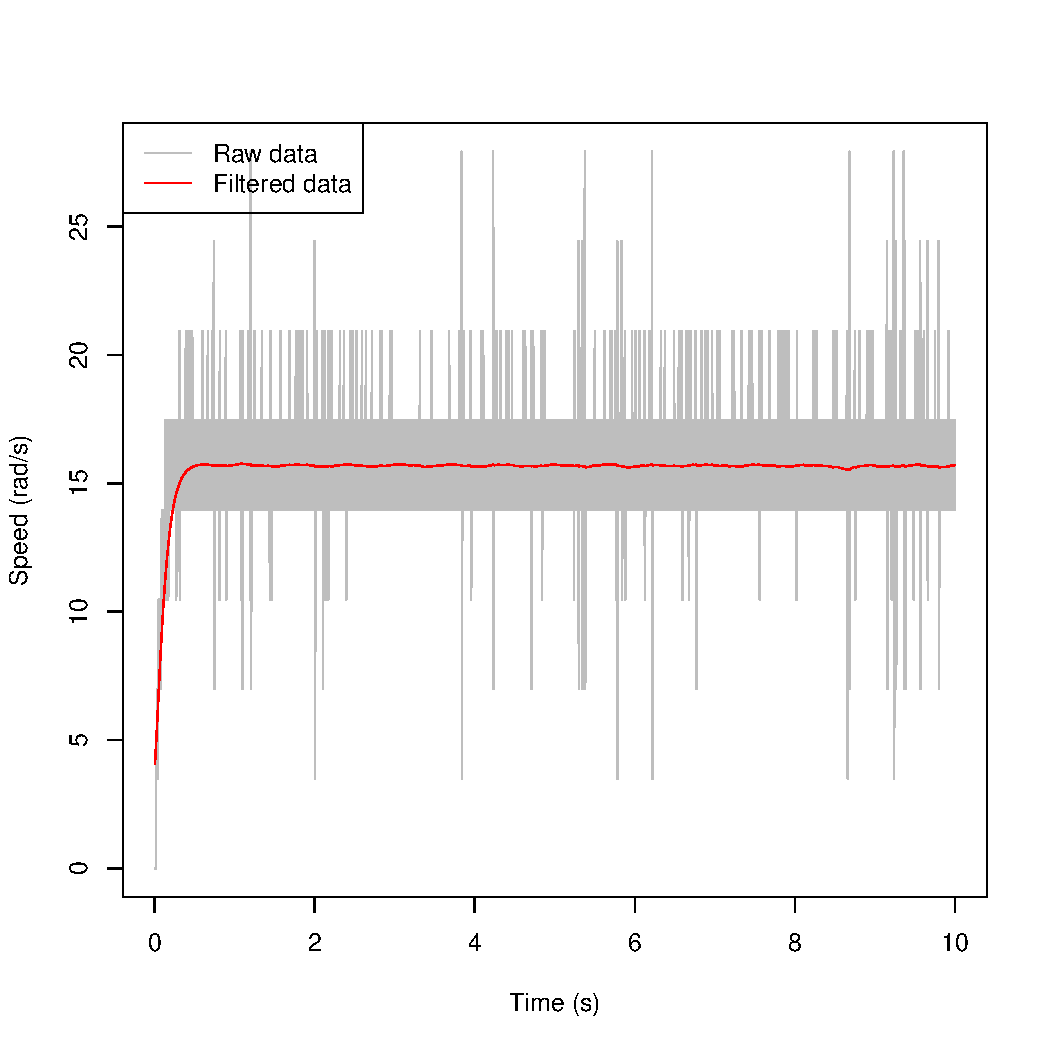
\includegraphics[width=\columnwidth]{../motor_data/plots/filtering/90}
	\caption{Root locus, blue lines show constains on overshot and settling time}
	\label{fig:root_locus}
\end{figure}

\begin{figure}[t]
	\centering
	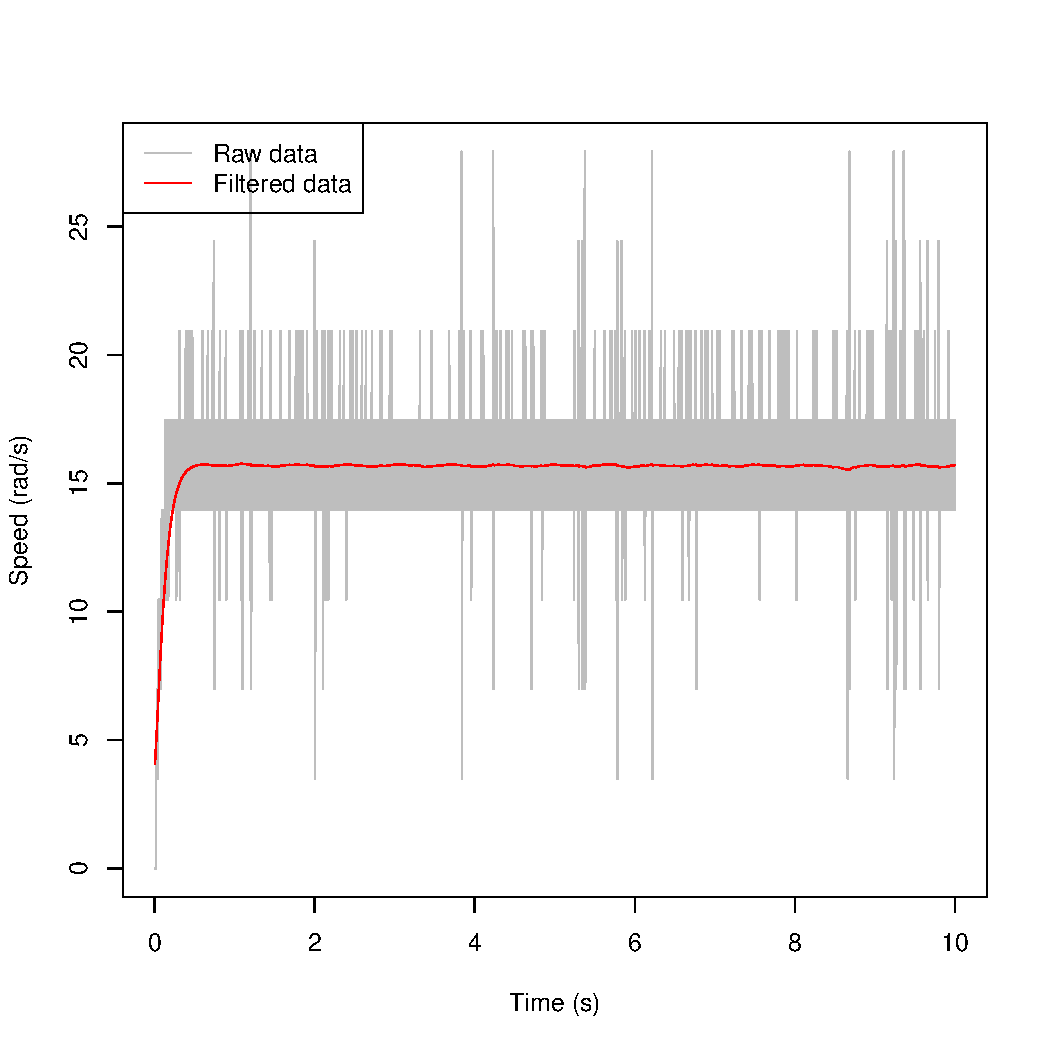
\includegraphics[width=\columnwidth]{../motor_data/plots/filtering/90}
	\caption{Responce to 1(t).}
	\label{fig:responce}
\end{figure}

\begin{figure}[t]
	\centering
	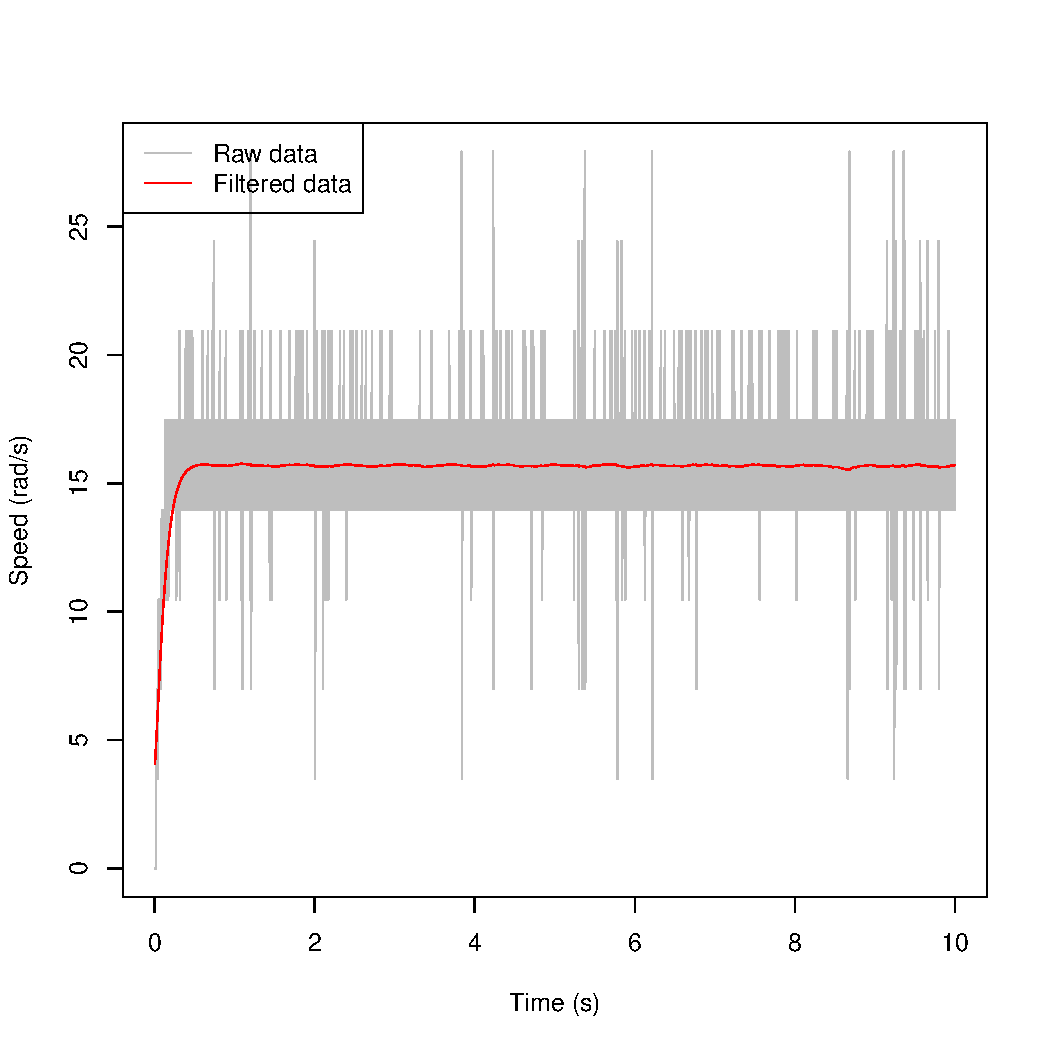
\includegraphics[width=\columnwidth]{../motor_data/plots/filtering/90}
	\caption{Scicoslab simulation.}
	\label{fig:simulation}
\end{figure}

\section{Implimentation of digital controller}
Digital vestion of controller is (obtained using trapezoid rule):
\begin{multline}
y_{k+2} = \frac{1}{4 + 42 * T} (K_cu_{k+2}(4 + 100T^2 + 40T) + K_cu_{k+1}(-8 + 200T^2) \\+ K_cu_{k}(4 - 40T + 100T^2) + 8y_{k+1} - y_{k}(4 - 42*T))
\end{multline}

\section{Conclusion}


\end{document}